% ============================================================
%  Figure 3 — Pickup bar chart: three states × three relays
%  Fixed | Local-Adaptive (pre-coord) | Coordinated (post-coord)
%  R_1, R_2, R_B
% ============================================================
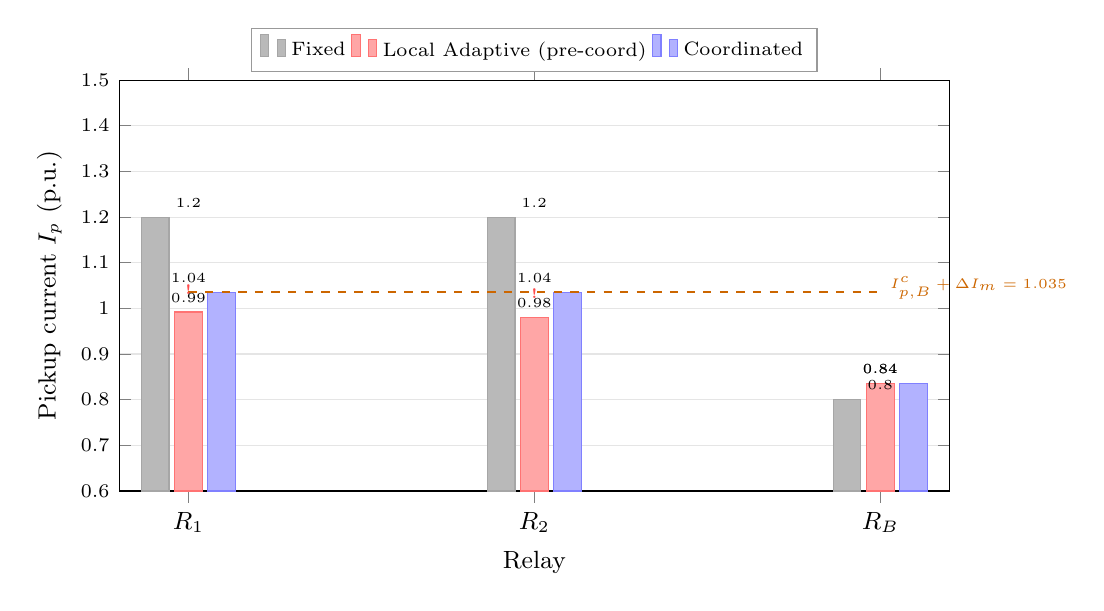
\begin{tikzpicture}
\begin{axis}[
  width=\columnwidth, height=6.8cm,
  ybar=5pt,
  bar width=10pt,
  xlabel={Relay},
  ylabel={Pickup current $I_p$ (p.u.)},
  symbolic x coords={$R_1$, $R_2$, $R_B$},
  xtick=data,
  x tick label style={font=\small},
  ymin=0.60, ymax=1.50,
  ytick={0.6,0.7,0.8,0.9,1.0,1.1,1.2,1.3,1.4,1.5},
  ymajorgrids=true, grid style={gray!20},
  label style={font=\small},
  tick label style={font=\scriptsize},
  legend style={at={(0.50,1.02)}, anchor=south,
                font=\scriptsize, fill=white, draw=black!40,
                legend columns=3},
  nodes near coords,
  nodes near coords align={vertical},
  every node near coord/.style={font=\tiny},
  clip=false
]

%% Fixed settings (dark gray)
\addplot[fill=gray!55, draw=gray!70, bar shift=-12pt] coordinates {
  ($R_1$,  1.200)
  ($R_2$,  1.200)
  ($R_B$,  0.800)
};

%% Local adaptive — pre-coordination (red, shows violation)
\addplot[fill=red!35, draw=red!55, bar shift=0pt] coordinates {
  ($R_1$,  0.992)
  ($R_2$,  0.980)
  ($R_B$,  0.835)
};

%% Coordinated (blue, restored)
\addplot[fill=blue!30, draw=blue!50, bar shift=12pt] coordinates {
  ($R_1$,  1.035)
  ($R_2$,  1.035)
  ($R_B$,  0.835)
};

%% Minimum selectivity margin reference line
%% I_p,B (coord) + delta_Im = 0.835 + 0.200 = 1.035
\draw[thick, orange!80!black, dashed]
      (axis cs:$R_1$,1.035) -- (axis cs:$R_B$,1.035);
\node[right, font=\tiny, orange!80!black]
      at (axis cs:$R_B$,1.045)
      {$I_{p,B}^c + \Delta I_m = 1.035$};

%% Violation markers on pre-coord bars
\node[font=\tiny, red!70!black, above] at (axis cs:$R_1$,1.01)
     {\textcolor{red!70}{\textbf{!}}};
\node[font=\tiny, red!70!black, above] at (axis cs:$R_2$,1.00)
     {\textcolor{red!70}{\textbf{!}}};

\legend{Fixed, Local Adaptive (pre-coord), Coordinated};
\end{axis}
\end{tikzpicture}
